\chapter{``Stochastic mitotic mode" models do not explain zebrafish retinal progenitor lineage outcomes}
\chaptermark{SMME models do not explain RPC lineage outcomes }
\label{chap:SMME}
\textit{The text of this chapter has been adapted from a manuscript originally prepared for submission to PLOS One and is formatted accordingly; the methods and supplementary materials are available in \autoref{sec:SMMsupp}}

\section{Introduction}

Mechanistic explanations (MEx) derive their utility from the resemblance of the conceptual mechanism's output to empirically observed outcomes. As maps to biological territories, biological MEx are habitually identified with the living systems they represent. Most well-developed MEx take the form of a model, whose internal structure is taken to reflect the underlying causal structure of a biological phenomenon. The nature of the causal relationship between a mechanistic model and the phenomenon it purports to explain remains a topic of active discussion in the philosophy of biology \cite{Fagan2015}. Biologists, nonetheless, usually accept that a model which explains empirical observations well (usually measured by statistical or information theoretic methods), and reliably predicts the results of interventions, bears a meaningful structural resemblance to the actual causal process giving rise to the modelled phenomenon.

Biological phenomena are notable for exhibiting both complex order and unpredictable variability. A significant challenge for MEx in multicellular systems is to explain how complex, highly ordered tissues, like those produced by neural progenitors, can arise from unpredictably variable cellular outcomes. Stem cell biologists have often used to Simple Stochastic Models (SSMs) in order to explain the observed unpredictable variability in clonal outcomes of putative stem cells \cite{Fagan2013}. Because SSMs are susceptible to Monte Carlo numerical analysis as Galton-Watson branching processes, they have been convenient explanatory devices, appearing in the literature for more than half a century \cite{Till1964}. By specifying the probability distributions of symmetric proliferative (PP), symmetric postmitotic (DD), and asymmetric proliferative/postmitotic (PD) mitotic modes, SSMs allow cell lineage outcomes to be simulated.

SSMs are ``stochastic" insofar as they incorporate parametric random variables. As Jaynes has noted, ``[b]elief ... that the property of being ‘stochastic' rather than ‘deterministic' is a real physical property of a process, that exists independently of human information, is [an] example of the mind projection fallacy: attributing one’s own ignorance to Nature instead." \cite{Jaynes2003} Despite this, macromolecular processes are often described as ``stochastic" in the stem cell literature. Generally speaking, the behaviour of an SSM's random variable is taken to represent sequences of outcomes that are produced by multiple, causally independent events. Recently, the influence of ``transcriptional noise" on progenitor specification has been identified as a candidate macromolecular process that may produce unpredictable variability in cellular fate specification. Therefore, one explanatory strategy for stem and progenitor cell function compares SSM model output to observed lineage outcomes, in order to argue that ``noisy", causally independent events give rise to the proliferative and specificative outcomes of progenitor lineages.

In this report, we evaluate the best-developed of these explanations, proffered by William Harris' retinal biology group. We have dubbed this the "Stochastic Mitotic Mode Explanation" (SMME) for zebrafish retinal progenitor cell (RPC) function. The SMME is noteworthy because it claims: (1) to "provid[e] a complete quantitative description of the generation of a CNS structure in a vertebrate in vivo" \cite{He2012}; (2) to have established the functional equivalency of embryonic RPCs and their descendants in the postembryonic circumferential marginal zone (CMZ) \cite{Wan2016}; and (3) to have established the involvement of causally independent transcription factor signals in the production of unpredictably variable RPC lineage outcomes \cite{Boije2015}. Moreover, the SMME is taken to supply evidence for the predominance of stochastic effects over other explanations for RPC lineage outcomes, such as the classical explanation of a temporal succession of competency states \cite{Temple1986}. These would be significant achievements with important consequences for both our fundamental understanding of CNS tissue morphogenesis and for retinal regenerative medicine. However, these models were not subjected to model optimization or selection procedures, as advocated by model selection theorists \cite{Burnham2002}, and widely adopted in ecology and evolutionary biology \cite{Johnson2004}.

In order to evaluate of the two SSMs which form the SMME's MEx for RPC function, we have re-expressed the models as cellular agent simulations conducted using the open source C++-based CHASTE cell simulation framework \cite{Mirams2013}. We explored the structure of the SSMs, dubbed the He and Boije SSM respectively, compared to their explanatory forebear, dubbed the Gomes SSM \cite{Gomes2011}. This analysis suggested the progression of temporal ``phases" in the models was largely responsible for the SMME model fits to data. In order to investigate this possibility, we built an alternative model with a deterministic mitotic mode and compared its output to the He SSM. We found that the deterministic alternative model was a better explanation for the observations, demonstrating that SMME fails when compared to alternatives. We therefore suggest that an explanatory approach based on the use of SSMs is incapable of distinguishing between theoretical alternatives for the causal structure of RPC lineage behaviours. Furthermore, by comparing the output of the models with novel postembryonic measurements of proliferative actvity, we find that the SMME explanation cannot account for quantitative majority of retinal growth in the zebrafish, driven by the CMZ. Finally, we discuss the place of SSMs, the concept of ``mitotic mode", and the role of ``noise" in explaining RPC behaviour, and suggest ways to avoid the modelling pitfalls exemplified by the SMME.

\section{Results and Discussion}

The SMME for zebrafish RPC function has been advanced using two SSMs. One first appears in He et al., and again, unmodified, in Wan et al. \cite{He2012,Wan2016}; it explains lineage population statistics and time-dependent rates of the three generically construed mitotic modes (that is, PP, PD, DD). We have called this the He SSM. The second appears in Boije et al. \cite{Boije2015}; its intent is both to introduce the role of specified macromolecules into the mitotic mode process, and to explain neuronal fate specification in terms of the process. We have called this the Boije SSM. The He model is directly descended an SSM advanced to investigate causally independent fate specification in late embryonic rat RPCs, formulated in Gomes et al. \cite{Gomes2011}. The Boije SSM differs substantially from the He and Gomes models, but inherits its general structure from the He SSM.

The metascientific analysis of the development of biological explanations remains undertheorized. Perhaps most refined tool for global evaluation of biological theories (Schaffner's "Extended Theories"), treats biological explanations as hierarchically organised logical structures, after the fashion of Imre Lakatos, and proposes the use of Bayesian logic to distinguish between them \cite{Schaffner1993}. However, biologists rarely offer explanations in this form; we rather prefer mechanisms, expressed in diagrammatic form or as mathematical model-objects.

In this report, we accept Fagan's view that MEx for the behaviour of stem and progenitor cells consist of assemblages (``mechanisms") of explanatory components which are understood to be causally organised by virtue of their intermeshing properties \cite{Fagan2015}. While Fagan treats SSMs seperately from macromolecular MEx, and we find that the Gomes SSM was not deployed in this role, the He and Boije SSMs were used as explanations for the behaviour of RPCs. As Feyerabend famously observed, scientists operate as epistemological anarchists; the development of our explanatory logic is not bound by a set of rules, but rather arises organically from our scientific objectives, extrascientific context, and so on \cite{Feyerabend1993}.
 
We have therefore chosen to examine the structure of the Gomes, He, and Boije SSMs arranged in chronological order, to highlight how the explanatory logic of zebrafish SMME SSMs differs from their immediate ancestor, and from other uses of SSMs in stem cell biology. We have diagrammatically presented these SSMs as MEx, consisting of components describing the proliferative and fate specification behaviour of cellular agents. The proliferative and specificative components of the MEx are causally organised by their Faganian intermeshing property, mitotic mode. We have used abbreviations to denote important classes of model components and inputs, informed by the emphasis of Feyerabend on the persuasive role of metaphysical ingredients and auxiliary scientific material; these are as follows:

 \begin{itemize}
	\item{MI - Model ingredient, making reference to some conceptual or metaphysical construct}
	\item{AS - Auxiliary scientific content}
	\item{RV - Random variable}
	\item{PM - Parameter measurement, model parameter set by measurements, independently of model output considerations}
	\item{PF - Parameter fit, model parameter set without reference to measurement, in order to produce model output agreement with observations}
\end{itemize}

We draw the reader's attention to the expansion of the ``mitotic mode'' intermeshing property in later SSMs; this explanatory component comes to dominate the later models, which makes its interpretation critical to the success of the mechanistic explanation in meaningfully representing a real biological process. 

Numerous explanations for variability in RPC lineage outcomes have been considered. Harris has argued that these belong to three cell-autonomous categories of process, in addition to extracellular influences: (1) a linear temporal progression of competency states, (2) asymmetric segregation of determinants during mitoses, and (3) intracellular ``stochastic events" \cite{Holt1988,Agathocleous2009}. All of the SSMs are used to argue for the predominant influence of the third type of process in RPC lineage outcomes, essentially by demonstrating that the output of the SSM resembles observations.
 
 \subsection{Gomes SSM: Ancestral Model of the SMME SSMs}
 
The Gomes SSM is presented in Fig \ref{GomesSSM}. The model's structure is straightforward; there are three independent random variables, drawing from empirically-derived probability distributions for the time each cell takes to divide, the mitotic mode of the division, and the specified neural fate of any postmitotic progeny. The random mitotic mode variable functions as the "intermeshing property" linking cycle behaviour to fate specification. In this scenario, the processes governing proliferation, leading to cell cycle exit, and governing cell fate commitment are causally independent of each other and of their history. The objective of the Gomes et al. study is to compare the lineage outcomes of dozens of individual E20 rat RPCs, in clonal-density dissociated culture, with the model output, developing earlier work in this system \cite{Cayouette2003}. Although the model incorporates conventional proper time (clock-time), none of the RVs reference it to determine their values. The abstract ``cells" represented by this model do not have any timer or any source of information about their relative lineage position.  Fate specification is construed in terms of conventional histochemical markers of stable cell fates; only the neural types generated late in the retinal histogenetic order are represented, as these are the only neurons specified by E20 rat RPCs.
 
  % Place figure captions after the first paragraph in which they are cited.
\begin{figure}[!h]
\makebox[\textwidth][c]{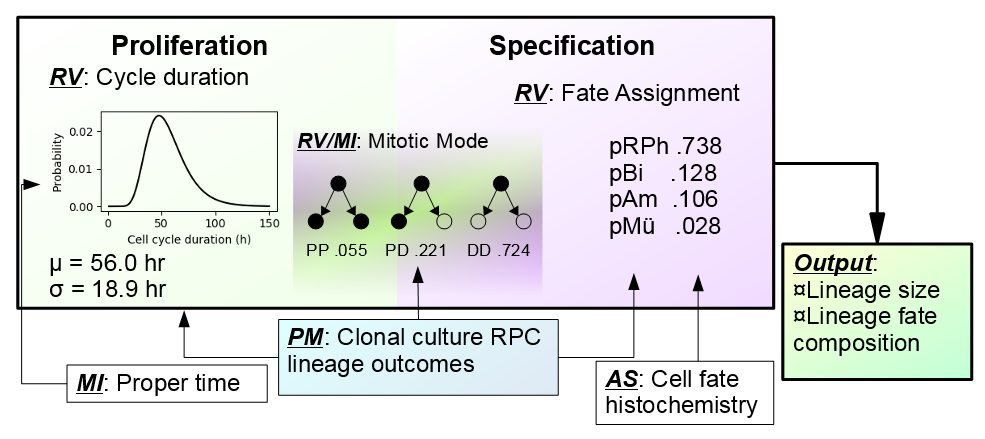
\includegraphics[width=1.2\textwidth]{ssm/Fig_1_Gomes.png}}
\caption{{\bf Structure of Gomes SSM}}
Structure of the Gomes SSM \cite{Gomes2011}. pRPh, probability of rod photoreceptor specification. pBi, probability of bipolar cell specification. pAm, probability of amacrine cell specification. pM{\"u}, probability of M{\"u}ller glia specification.
\label{GomesSSM}
\end{figure}
 
This SSM is explicitly built as a null hypothesis, or a model of background noise. It represents an extreme case in which all of the specificative and proliferative behaviours of an RPC are totally independent of all other RPCs and events in its clonal lineage. The stated purpose of this model is ``to calibrate the data", serving ``as a benchmark" \cite{Gomes2011}, a purely hypothetical apparatus to produce sequences of causally unrelated lineage outcomes. Substantial deviations of the observed data from the fully independent events of the SSM may then be interpreted as causal dependencies between RPC outcome and their relative lineage relationships, as might be observed in a developmental ``program" or algorithmic process. Finding that, with some exceptions, observed proliferative and specificative outcomes generally fall within the plausible range of Gomes SSM output, Gomes et al. conclude that RPC lineage outcomes in late embryonic rat RPCs seem to be dominated by causally independent events, suggesting that causally isolated ``noisy" macromolecular processes may give rise to the unpredictable variability in the fate outcomes of these cells. 
 
 \subsection{He SSM: Explaining variability in zebrafish neural retina lineage size}
 
The He SSM, shown in Fig \ref{HeSSM}, is deployed in a explanatory role rhetorically identical to the Gomes SSM. The extent to which model output ``captures.. aspects of the data" is taken to obviate the need for explicit ``causative hypothes[e]s". On this account, only residual error between model output and observations may be ascribed to non-stochastic processes like ``histogene[tic ordering] of cell types or a signature of early fate specification". That is, if the model can be fit to observations, this is taken to exclude the presence of any cell-autonomous temporal program, asymmetric segregation of fate determinants, extracellular influences, and the like. 

  % Place figure captions after the first paragraph in which they are cited.
\begin{figure}[!h]
\makebox[\textwidth][c]{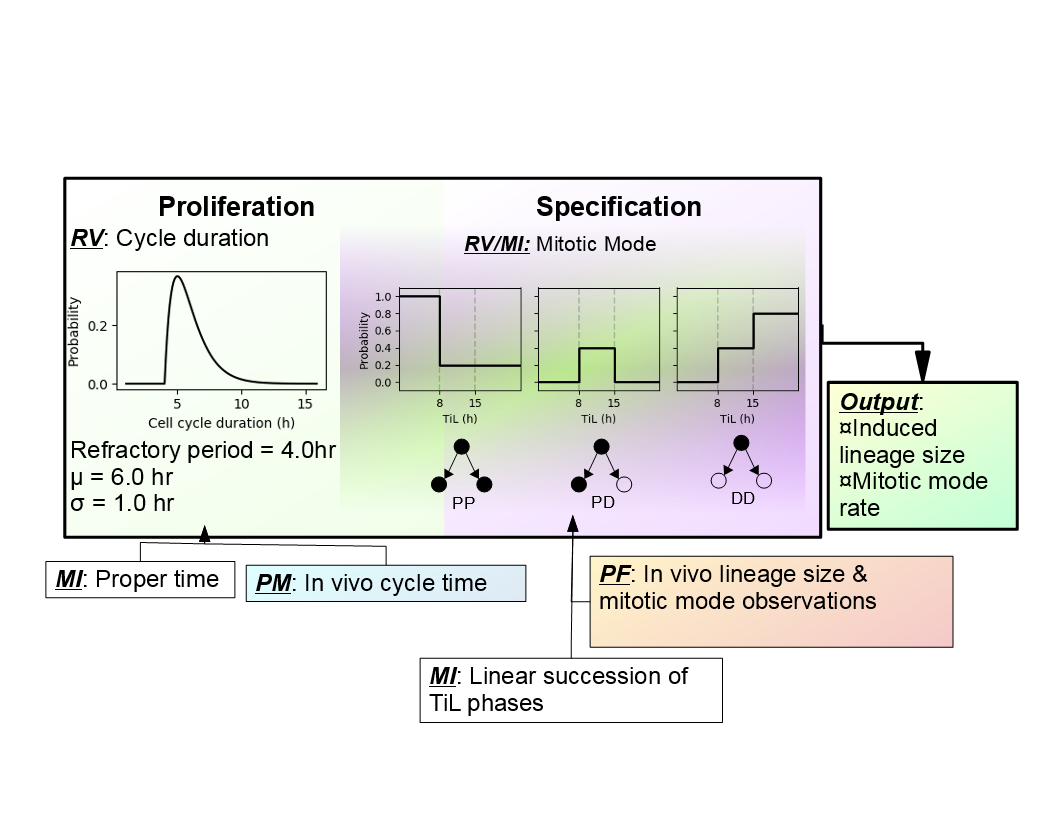
\includegraphics[width=1.2\textwidth]{ssm/Fig_2_He.png}}    
\caption{{\bf Structure of He SSM}}
Structure of the He SSM \cite{He2012}. TiL, Time in Lineage.
\label{HeSSM}
\end{figure}

There are fewer direct empirical inputs to the He model's parameters than the Gomes SSM, limited to the duration of the cell cycle. The close synchrony of zebrafish RPC divisions is modelled by assigning sister RPCs the same cycle length, shifted by a normal distribution with a variance of one hour, in contrast to Gomes RPCs, which are treated as fully independent. The lineage outcomes the He SSM is called on to explain differ significantly from those referred to by the Gomes SSM. Most notably, the Gomes SSM does not account for the early appearance of RGCs, which are not produced by the late E20 progenitors examined in that study. The zebrafish RPC lineages studied by He et al. produce all of the retinal neural types, including RGCs, which are typically produced by PD-type divisions. The He SSM does not model particular cell fates, supposing that mitotic mode is ``decoupled" from fate specification. The mitotic mode RV linking cell cycle to fate specification in the Gomes SSM has thus subsumed the specification outcomes of RPC lineages entirely, and the model is concerned only to explain the sizes of lineages (marked by an inducible genetic marker at various times), and the observed progression of mitotic modes in these early RPCs.

The He model is, therefore, called on to explain the temporal structure of the proliferative behaviour of early zebrafish RPCs that dissociated late rat RPCs do not exhibit. A Gomes-type SSM, in which the RVs determining RPC behaviour are independent of any measure of time, cannot account for this temporal progression. In order to address this, He et al., assume a linear progression of three phases which cells in each lineage pass through, the timing of these phases being determined relative to the first division of the RPC lineage, called here ``Time in Lineage" or TiL. The parameters of the mitotic mode RV are determined by these TiL phases. The temporal structure of the phases and their effect on the mitotic mode RV are selected to produce a model fit. While He et al. acknowledge that the model therefore represents a ``combination of stochastic and programmatic decisions taken by a population of equipotent RPCs," no test is performed to determine the relative contribution of the model's stochastic vs. linear programmatic elements. Instead, the purportedly stochastic nature of mitotic mode determination is emphasized throughout the report.

 \subsection{Boije SSM: Explaining variability in zebrafish RPC fate outcomes}
 
The second SMME model advanced to explain zebrafish RPC behaviour, the Boije SSM, is diplayed in Fig \ref{BoijeSSM}. This model is primarily concerned with the lineage fate outcomes that the He SSM does not treat, while abandoning the explicit proper time of the He and Gomes SSMs in favour of abstract generation-counting. The mitotic mode model-ingredient now subsumes all RPC behaviours. Boije et al. make a laudable effort to specify the particular macromolecules ostensibly involved in determining mitotic mode, nominating the transcription factors (TFs) Atoh7, known to be involved in RGC specification, and Ptf1a, known to be involved in the specification of amacrine and horizontal cells, as primary candidates. The contribution of vsx2 is taken to determine the balance between PP and DD divisions late in the lineage, with the latter resulting in the specification of bipolar or photoreceptor cells. The binary presence or absence of these signals is determined by independent RVs structured by the phase structure present in the He SSM, translated into generational time from proper time.

\begin{figure}[!h]
\makebox[\textwidth][c]{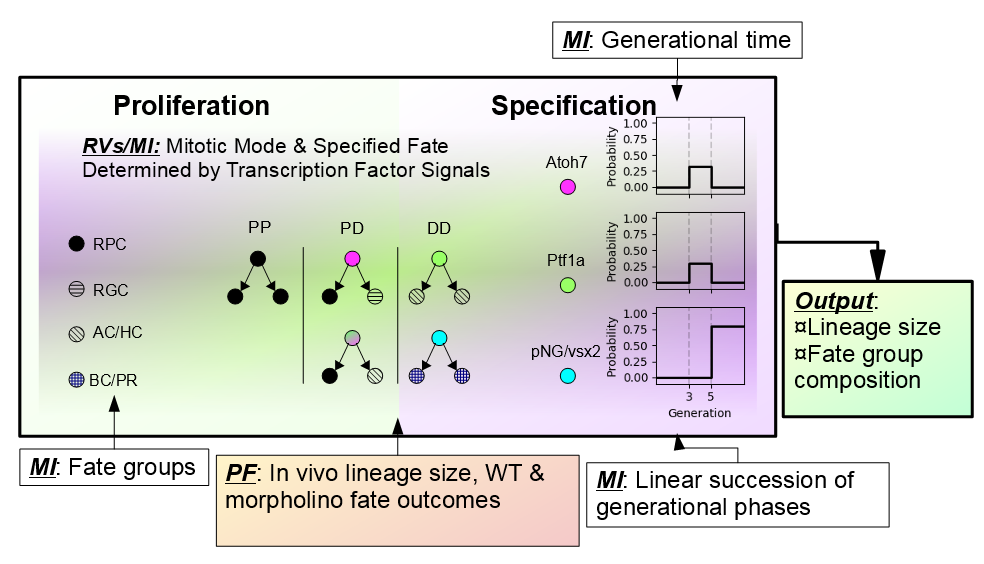
\includegraphics[width=1.2\textwidth]{ssm/Fig_3_Boije.png}}
\caption{{\bf Structure of Boije SSM}}
Structure of the Boije SSM \cite{Boije2015}. RPC, retinal progenitor cell. RGC, retinal ganglion cell. AC, amacrine cell. HC, horizontal cell. BC, bipolar cell. PR, photoreceptor. pNG- parameter representing contributions of Vsx1 and Vsx2 to specification of BC \& PR fates in absence of Atoh7 or Ptf1a signals.
\label{BoijeSSM}
\end{figure}

By this point, the SMME has become a very different type of explanation from its Gomes SSM forebear. We are no longer dealing with RVs that model causally and temporally independent processes for different aspects of RPC behaviour. There is, rather, one temporally dependent process, the determination of mitotic mode, which is explained by unpredictable subsets of each lineage generation expressing particular TF signals. Where the Gomes SSM takes its parameters directly from empirical measurements of lineage outcomes, asking whether it is sufficient to assume that these are independently determined, the Boije SSM's parameters are derived solely from model fit considerations. In spite of these considerable differences, the explanatory role of the SSM is effectively the same: the model's fit to observations is taken as evidence of the predominant influence of stochastic processes determining mitotic mode on RPC behaviour. While Boije et al. acknowledge that whether some process is called ``deterministic" or ``stochastic" is ``a matter of the level of description" \cite{Boije2015} (i.e. is a property of the model-description and not of the physical process), the explanatory role of stochasticity for RPC lineage outcomes is emphasized throughout.
 
 \subsection{Model selection demonstrates the SMME is not the best available explanation for RPC lineage outcomes}
 
From a modeller's perspective, it is notable that neither of the reports which use the He SSM \cite{He2012,Wan2016}, nor that using the Boije SSM \cite{Boije2015} report in any detail their fitting procedures, nor do any of the above report any statistical measures of goodness-of-fit. Additionally, no models representing the alternative ``theoretical options" available to explain variability in RPC lineage outcomes are compared to those advanced as evidence for stochastic processes. Given that the He SSM and Boije SSM depart from the Gomes SSM by the addition of an unexplained temporal structure to the mitotic mode model ingredient, it is striking that the overall argument remains similar to Gomes et al.'s, despite the persuasive force of the latter deriving from the lack of such structures. While He et al. and Boije et al. acknowledge that their models involve both stochastic and linear programmatic elements, their relative influence on model output is not measured, and macromolecular explanation is only applied to the stochastic elements. Moreover, the emphasis on this mitotic mode model construct increases with each successive model, to the extent that in the Boije model there are no other elements that are used to explain RPC behaviours. All cellular behaviours are, in effect, progressively collapsed into the stochastic mitotic mode concept. Finally, the He and Boije SSMs contain more parameters, which are determined by fewer empirical measurements than the Gomes SSM. It is therefore important to test whether the most important ingredient in these models is the stochastic mitotic mode, against the possibility the unexplained temporal structure is the truly explanatory element.

Fortunately, we may employ model optimisation and selection techniques to adjudicate this. The most straightforward way to do so is to reexamine the He SSM alongside a competing alternative model. The data to which the He SSM has been applied is amenable to a scheme in which the models are fit to a ``training" dataset, followed by a ``test" dataset. In this case, the training data are the induced lineage size and mitotic mode rate data from He et al. The test dataset comprises the Atoh7 morpholino observations from He et al., and the CMZ lineage size data from Wan et al. This allows us to test how well the He SSM, and an alternative, hold up under novel experimental conditions, without relying on a trivial ordering of goodness-of-fit to training data. Since the Boije SSM draws straightforwardly on the He SSM for its temporal phase-parameterisation and stochastic mitotic mode model ingredient, this analysis of the He SSM also bears directly on the validity of the Boije SSM.

As an alternative to the SMME He SSM, we constructed a model that has a deterministic mitotic mode with variable phase lengths. Rather than variability arising from a stochastic-process mitotic mode changing across phases of fixed length, we simply supposed that mitotic mode is deterministic in each phase (guaranteed PP mitoses in the first phase, PD in the second, and DD in the third), but the phase lengths are variable between lineages and shift slightly between sister cells. That is, we represented this linear progression of deterministic mitotic mode phases using the same type of statistical construct the He SSM applies to model cell cycle length, to avoid introducing any novel or contentious elements into the model comparison. More specifically, each lineage has a first PP phase length drawn from a shifted gamma distribution, followed by a second phase length drawn from a standard gamma distribution. Upon mitosis, these phase lengths are shifted in sister cells by a normally distributed time period, exactly like cell cycle lengths in the He SSM.

We take this to be a reasonable representation of the classic suggestion that RPCs step through linear succession of competency phases, given the conceptual tools that the He SSM uses to model mitotic phenomena. If we suppose that this temporal program is governed by RPC lineages passing through a stereotypical series of chromatin configurations which allow for PP, then PD, then DD mitoses in turn, along with the associated competence to produce the particular cell fates associated with PD and DD mitoses, it seems entirely plausible to suggest that lineages differ in the lengths of time they occupy each state. This is particularly true if we concede that an SSM, foregoing any spatial modelling whatsoever, must necessarily abstract extracellular and spatial influences on these processes. Moreover, since these chromatin configurations must be broken down and rebuilt with each mitosis, the re-use of the ``sister shift" model ingredient from the He SSM's cell cycle RV is congenial, representing the same sort of cell-to-cell variability that results in the small differences between sister cells in cycle timing. 

While the code used to implement the SSMs mentioned above has not been published, the relevant reports provide enough detail to reconstruct these models in full, which we did using the CHASTE cell-based simulation framework, in order to provide transparent and reproducible implementations of the SSMs. Because the values selected for the He SSMs' parameters seem to have been selected as a series of rough estimates, with only the value for the probability of PD-type mitoses in the second model phase being varied to produce the fit, we suspected that the fit would not be at or near the local minimum for a loss function. That is, a model fit produced in this manner is likely to be located in a region of the parameter space that is highly sensitive to small perturbations, and therefore may depend strongly on implementation-specific idiosyncracies. He et al. report that they experienced difficulty in obtaining a good fit to their 32 hour induction data, with changes in the phase two PD probability producing large differences in fit quality. Unsurprisingly, when we rebuilt the He SSM with the original fit parameterisation, we substantially reproduced the original fit, except for the 32 hour data, where the model output diverges substantially from that reported in He et al. (see \nameref{originalSupplement}). Since this is clearly not the best fit available for the He SSM, and we wish to directly compare the best fits (i.e. the parameterisations at minima of some loss function) for the He SSM and our putative alternative model, we used the simultaneous perturbation stochastic approximation (SPSA) algorithm \cite{Spall1998} to optimise both models against test data. SPSA is particularly convenient for complex, multi-phase models like the He SSM, because no knowledge of the relationship between the model's parameters and the loss function is required. We used Akiake's information criterion (AIC) as the loss function to be minimised, in order to provide a rigorous comparison between the two differently-parameterised models (the deterministic alternative has two fewer parameters than the He SSM). 

\begin{figure}[p]
	\makebox[\textwidth][c]{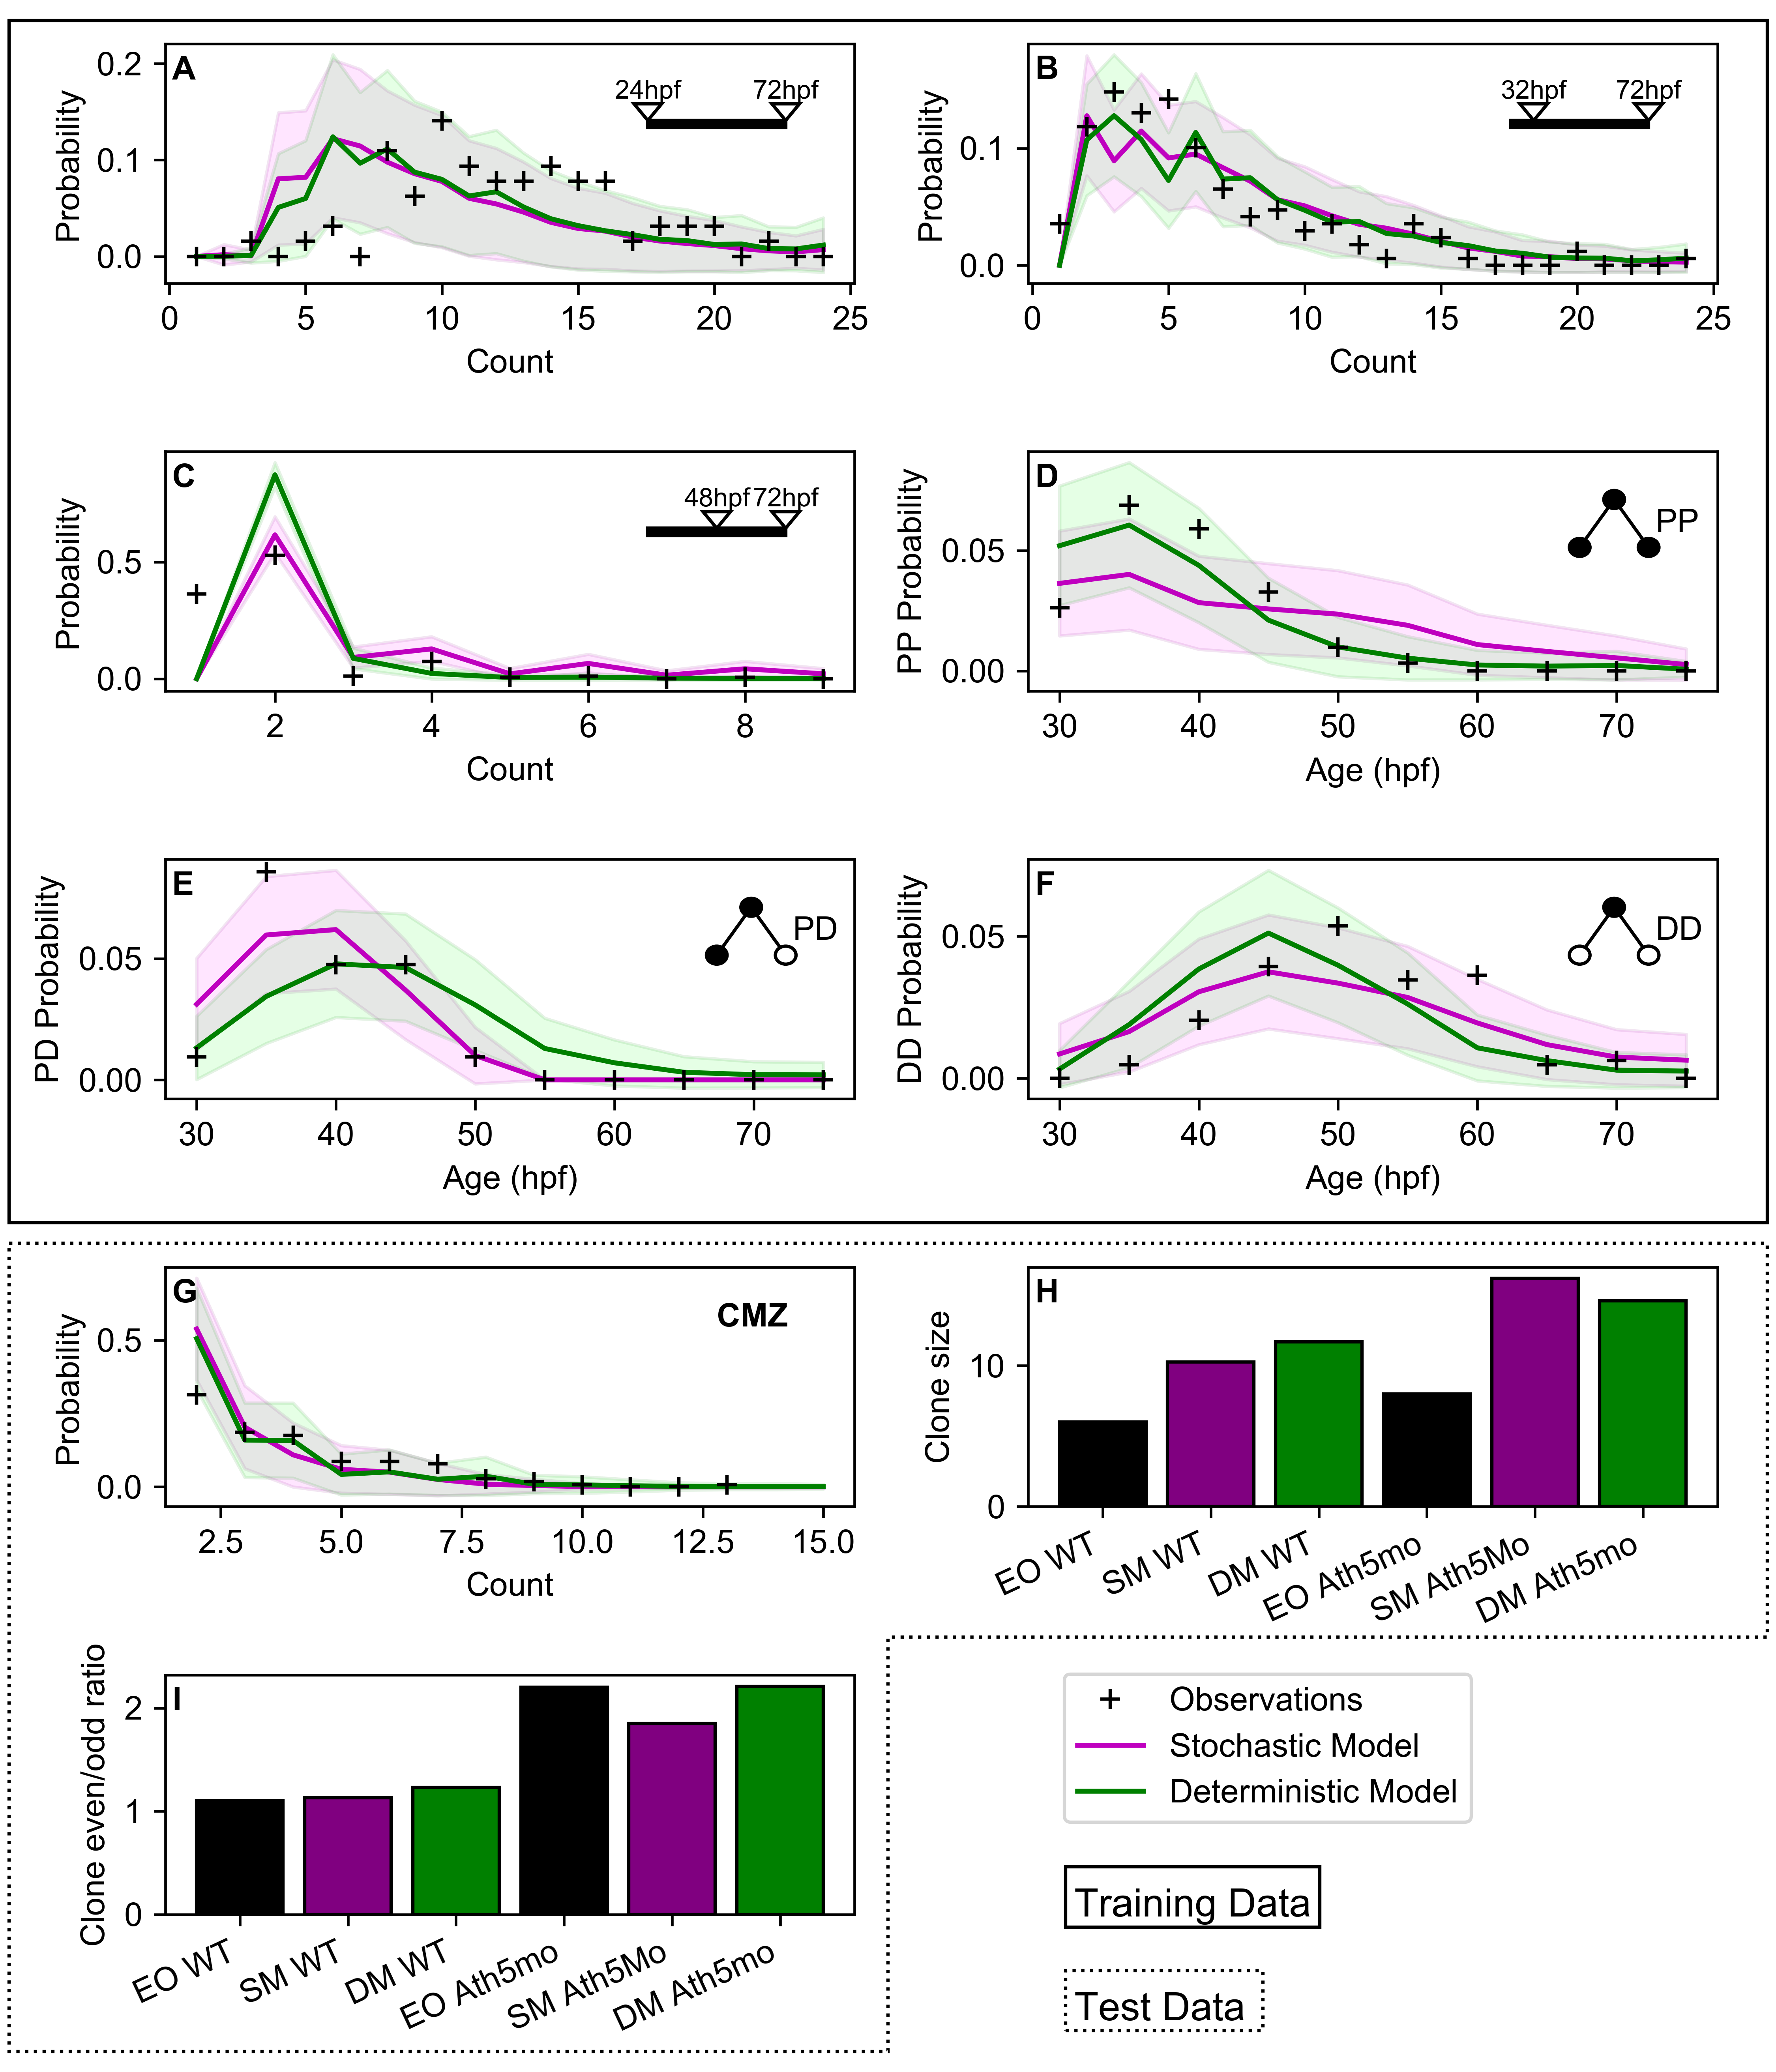
\includegraphics[width=1.\textwidth]{ssm/Fig_4_model_comparison.png}}
\caption{{\bf Model comparison: the SPSA-optimised He SSM and a deterministic alternative}}
Empirical observations (black crosses and bars) and SPSA-optimised model output (magenta, stochastic mitotic mode model; green, deterministic mitotic mode model). Model output in panels A-G is displayed as mean $\pm$ 95\% CI. Panels A-F: Training dataset, to which models were fit. Panels A-C: Probability of observing lineages of a particular size ("count") after inducing single RPC lineage founders at (A) 24, (B) 32, and (C) 48 hours with an indelible genetic marker, tallying their size at 72hpf. Panels D-F: Probability density of mitotic events of modes (D) PP, (E) PD, and (F) DD over the period of retinal development observed by He et al. Panel G: Probability of observing lineages of a particular size ("count") originating from the CMZ; RPCs are taken to be resident in the CMZ for 17 hours before being forced to differentiate, lineage founders are assumed to be evenly distributed in age across this 17 hour time period. Panel H: Average clonal lineage size of wild type and Ath5 morpholino-treated RPCs. Ath5mo treatment is taken to convert 80\% of PD divisions, which occur in the second phase of the He model, to PP divisions, resulting in larger lineages. Panel I: Ratio of even to odd sized clones in wild type and Ath5 morpholino-treated RPCs.
Methods in \autoref{ssec:CHASTEsims}.
Code in \autoref{ssec:He_output_plot}.
\label{SDFig}
\end{figure}
\FloatBarrier

After fitting to the training dataset, we calculated AIC for the He SSM (hereafter SM, for stochastic model) and our deterministic mitotic mode alternative (hereafter DM), for both training and test datasets. The combined results are displayed in Fig \ref{SDFig}, with the output of the two models being presented separately in \nameref{stochasticSupplement} and \nameref{deterministicSupplement}. Remarkably, the DM closely recapitulates the output of the SM for both datasets. Moreover, while the more highly-parameterised SM permits a better fit to the training data, the DM proves to be a better fit to the test dataset, as summarised in Table \ref{AICtable}. This can be understood as a case of model overfitting: a higher-parameter model fits some training dataset better than a simpler model, but fails upon challenge with a new dataset. Given this model selection scheme, it is plain that we should choose the DM over the SM as a superior explanatory model, both on the basis of explanatory power and of Occam's Razor.

\begin{table}[!ht]
\centering
\caption{
{\bf AIC values for models assessed against training and test datasets}}
\begin{tabular}{|l|l|l|}
\hline
{\bf Model} & {\bf Training AIC} & {\bf Test AIC} \\ \hline
Stochastic (He fit) & -93.26 & 255.64\\ \hline
Stochastic (SPSA fit) & {\bf -93.80} & 92.24\\ \hline
Deterministic (SPSA fit) & -69.33 & {\bf 86.60}\\ \hline
\end{tabular}
\begin{flushleft} AIC: Akiake's information criterion. Lower values reflect better model explanations of the noted dataset. Lowest values are noted in bold.
Methods in \autoref{ssec:CHASTEsims}.
Code in \autoref{ssec:He_output_plot}.
\end{flushleft}
\label{AICtable}
\end{table}

We therefore conclude that the SMME is not the best available explanation for variability in zebrafish RPC lineage outcomes. It is clear from this analysis that the assumed, but unexplained, linear succession of mitotic mode phases is what provides the overall structure of the model output. Variability in lineage outcomes may be supplied by entirely different model ingredients without any loss of explanatory power on new datasets (indeed, with some improvement, in our case). To conclude that these models support a stochastic process governing mitotic mode, ruling out other types of explanation, is unjustified. It is likely that any number of different types of SSMs, representing other sorts of processes (such as asymmetric segregation of fate determinants, or differential spatial exposure to extracellular signals), can produce identical model output. Given this, we conclude that SSM models of this type are inadequate for the task of locating the source of variability in RPC lineage outcomes.

\subsection{SMME SSMs cannot explain the post-embryonic phase of CMZ-driven zebrafish retinal formation}

The zebrafish retina, like other fish retinas, and unlike the mammalian retina, continues to grow long after the early developmental period, indeed, well past the organism's sexual maturity. This may be unsurprising, given that zebrafish increase in length almost ten-fold over the first year of life \cite{Parichy2009}, necessitating a continuously growing retina during this period. In fact, the quantitative majority of zebrafish retinal growth occurs post-metamorphosis, outside of the early developmental period. This growth occurs due to the persistence of a population of proliferative RPCs present in an annulus at the periphery of the retina, called the ciliary or circumferential marginal zone (CMZ), which plates out the retina in annular cohorts. A typical "tree-ring" analysis from our studies, marking the DNA of cohorts of cells contributed to the retina at particular times with indelible thymidine analogues, is shown in Fig \ref{RingFig}. These experiments show the structure of the adult zebrafish retina is quantitatively dominated by contributions from the CMZ in the period between one and three months of age. Why peripheral RPCs in zebrafish remain proliferative, while those in mammals are quiescent \cite{Tropepe2000}, and whether and how their behaviour might differ from embryonic RPCs, remain unresolved. Answers to these questions may have significant fundamental and therapeutic implications, especially given e.g. the possibility of harnessing endogenous, quiescent, peripheral RPCs in humans for regenerative retinal medicine.

\begin{figure}[!h]
\makebox[\textwidth][c]{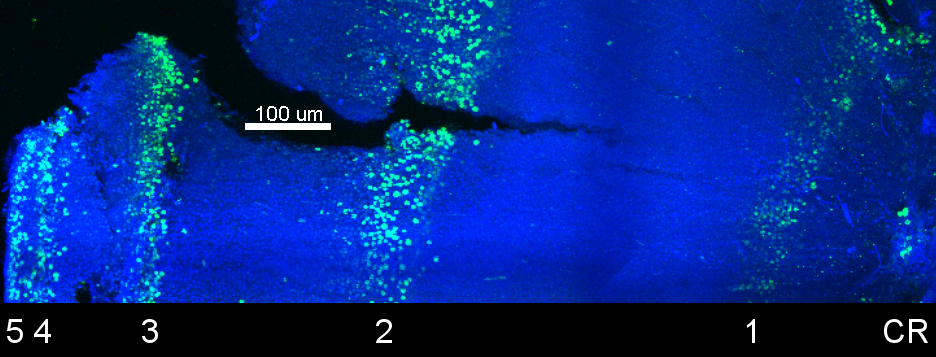
\includegraphics[width=1.\textwidth]{ssm/Fig_5_CMZ_cohorts.png}}
\caption{{\bf Most zebrafish retinal neurons are contributed by the CMZ between one and three months of age}}
Maximum intensity projection derived from confocal micrographs of a zebrafish whole retina dissected at 5 months post fertilisation (mpf). The animal was treated with BrdU at 1, 2, 3, 4, and 5 mpf for 24hr. Anti-BrdU staining of the whole retina reveals the extent to which the CMZ (which is responsible for retinal growth after approximately 72hpf) contributes new neurons in tree-ring fashion, extending out from the center of the retina (CR), which is formed before 72hpf. Monthly cohorts are labelled appropriately. Scale bar, 100 $\mu$m.
Methods in \autoref{ssec:SMMEwholeretina}.
\label{RingFig}
\end{figure}

\FloatBarrier

The He SSM was deployed in Wan et al. \cite{Wan2016}, with the claim that the He SSM explains the behaviour of CMZ RPCs. Wan et al. argue that a slowly mitosing population of bona fide stem cells, at the utmost retinal periphery, divides asymmetrically to populate the CMZ with He-SSM-governed RPCs. In other words, the usual suggestion that CMZ RPCs undergo a somewhat different process than embryonic RPCs, perhaps recapitulating across the peripheral-central axis some progression of states or lineage phases that embryonic RPCs pass through in time \cite{Harris1998}, is repudiated in favour of one model which describes the behaviour of all RPCs throughout the life of the organism, with the addition of a small population of stem cells to keep the CMZ stocked with RPCs. If so, this might suggest that the problem of activating quiescent stem cells in the retina is simply that- one need only sort out how to throw the proliferative switch in these cells, since the proliferative and fate specification behaviours of the resultant RPCs will reliably be the same as those observed in development.

While we determined that the SMME is not the best available explanation for RPC lineage outcomes, we still felt that the SSMs associated with this explanation might be used to elucidate this point. In particular, if it is the case that the He SSM provides good estimates of lineage size and proliferative dynamics in the early zebrafish retina, it should be possible, using this model, and the estimates of putative stem cell proliferative behaviour provided by Wan et al., to simulate the population dynamics of the CMZ, at least through the first few weeks of the organism's life.

In pursuing this point, we noted a peculiar feature of the He SSM not documented by any of the SMME reports: the cell cycle model overstates the  \textit{per-lineage} rate of mitoses by as much as a factor of 3. That is, the mitotic mode rate data presented in He et al., recapitulated here in Fig \ref{SDFig}, panels D, E, and F, and used to optimise both the SM and DM, are probability density functions that are not standardised on a per-lineage basis. These data simply indicate the distribution of mitotic events of a particular type. When we take all of the mitotic events documented by He et al. and calculate the probability of any such event occuring per lineage, per hour, we obtain the values presented in Fig \ref{PerLineageFig}.

\begin{figure}[!h]
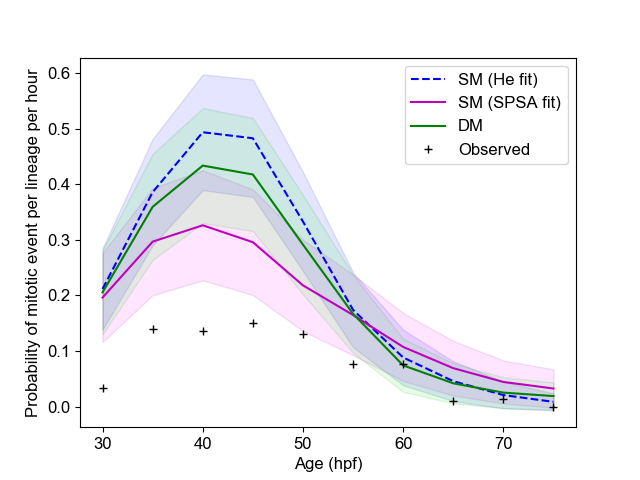
\includegraphics{ssm/Fig_6_per_lineage_mitotic_rate.png}
\caption{{\bf Per-lineage probabilities of mitoses, He et al. observations compared to model output}}
Probability of observing a mitotic event over the period studied by He et al., per hour, per lineage. Model output is presented as mean $\pm$ 95\% CI.
Methods in \autoref{ssec:CHASTEsims}.
Code in \autoref{ssec:Mitotic_rate_plot}.
\label{PerLineageFig}
\end{figure}

Similarly, when we performed cumulative thymidine analogue labelling of the 3dpf CMZ, (using the assumptions of Nowakowski et al. \cite{Nowakowski1989}, which treat the proliferating population as a homogenous, and dividing asymmetrically; these assumptions are flawed but adequate for a rough estimate) we obtain an average cell cycle length of approximately 15 hours, more than twice as long as the He SSM's mean cycle length. These data are displayed in \ref{cumulativeSupplement}. Therefore, the He SSM (in both its original and refit parameterisation, as well as the deterministic alternative, since they all rely on the same proliferative model elements) substantially overstates the proliferative potential of both embryonic and early CMZ RPCs. Since we observed a massive build-up of proliferating RPCs between two and four weeks post-fertilisation, we thought this might actually suit this later context better.

To estimate of total annular CMZ population in zebrafish retinas over time, we counted proliferating RPCs present in central coronal sections of zebrafish retinas throughout the first year of life, treating these as samples of the annulus, and calculated the total number of cells that would be present given the diameter of the spherical lens measured at these times. Our simulated CMZ populations were constructed at 3dpf by drawing an initial population of RPCs governed by the He SSM (using the original fit parameters, which further exaggerate the proliferative potential of these lineages) from the observed distribution. We added immortal stem cells amounting to one tenth of this total. This is likely an overestimate, given that these putative stem cells are thought to be those in the very peripheral ring of cells around the lens, of which typically two to four may be observed in our central sections with an average of over one hundred proliferating RPCs. Moreover, these simulated stem cells were given a mean cycle time of 30 hours, proliferating about twice as quickly as Wan et al. suggest. Finally, to reflect the fact that these stem cells contribute to the retina in linear cohorts \cite{Centanin2014}, and more of them are therefore required as the retina grows, the stem cells were permitted to divide symmetrically when necessary to maintain the same density of stem cells around the annulus of the lens. Two hundred such CMZ populations were simulated across one year of retinal growth.

The results of these simulations are displayed in Fig \ref{WanSim}, overlaid over CMZ population estimates derived from observations. Given the generous parameters of the population model, consistently overestimating the proliferative potential of embryonic and early CMZ RPCs, it is surprising that the He SSM proves completely unable to keep up with the growth of the CMZ in the first two months of life. Indeed, the unrealistically active stem cell population the simulated CMZs are provided with is unable to prevent a near-term collapse in RPC numbers, only catching up after the months later as the number of stem cells increases with the growth of the lens. Thus, even given permissive model parameters, the He SSM is not able to recapitulate the quantitatively most important period of retinal growth in the zebrafish.

\begin{figure}[!h]
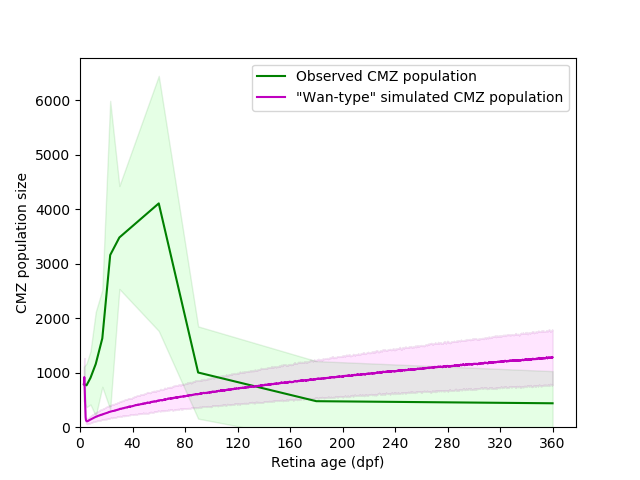
\includegraphics{ssm/Fig_7_wan.png}   
\caption{{\bf CMZ population of proliferating RPCs: estimates from observations and simulated Wan-type CMZs}}
Annular CMZ population was estimated from empirical observations of central coronal cryosections stained with anti-PCNA, a marker of proliferating cells, standardising by the diameter of the spherical lens observed in these animals. "Wan-type" CMZs were initialised with a number of RPCs drawn from from the observed 3dpf population distribution, and given an additional 1/10\textsuperscript{th} of this number of immortal, asymmetrically dividing stem cells, as described in the text, and simulated for the first year of life. All data is presented as mean $\pm$ 95\% CI.
Methods in \autoref{ssec:PCNA}, \autoref{ssec:CHASTEsims}.
Code in \autoref{ssec:Wan_output_plot}.
\label{WanSim}
\end{figure}

This analysis suggests that observations of RPCs in embryogenesis and early larval development are unlikely to provide a good quantitative model of the development of the zebrafish retina, even abstracting away spatial and extracellular factors as SSMs necessarily do. Our data point to a second, quantitatively more important phase of retinal development, between approximately one and four months of age, in which RPCs are far more proliferatively active than in early development. It is likely that models that closely associate proliferative behaviour with fate specification, like those of the SMME, will be unable to explain this period. Recent evidence suggests that mitotic and fate specification behaviours in RPCs may be substantially uncoupled \cite{Engerer2017}. This would permit the CMZ population to scale appropriately with the growing retina. Alternatively, it is possible that RPCs have heterogenous proliferative behaviour, and that this heterogeneity is mainly apparent later in development.

\section{Conclusion}

Simple stochastic models are familiar tools for stem cell biologists. Introduced by Till, McCulloch, and Siminovitch in 1964 \cite{Till1964}, they proved their utility in describing variability in clonal lineage outcomes of putative stem cells, originating from macromolecular processes beyond the scope of cellular models (and beyond the reach of the molecular techniques of the time). More prosaically, their simplicity afforded computational tractability in an era when processing time was relatively scarce, allowing early access to Monte Carlo simulation techniques. That said, their abstract nature emphasizes an aspatial, lineage-centric view of tissue development, which cannot account for the generation of structurally complex tissues like retinas beyond cell numbers, and, perhaps, fate composition. As a result of this relatively loose relationship to the complex morphogenetic environment, there are few constraints on the model configurations that may produce similar outputs. This can result in modellers being led astray by their apparently good fits to observations, which is why the fit of one highly parameterised model cannot be taken, alone, as evidence for some theory; it is very rare that there is not a model representing an alternative theory that cannot be made to produce a reasonable model fit. Indeed, as we demonstrate here, the use of standard model selection techniques may make plain that a completely contradictory theory is a better explanation for the data.

To some extent, this can be ameliorated by careful attention to the particular macromolecular or cellular referents that particular model constructs represent. The ``mitotic mode" construct present in all SSMs is a particularly ambiguous and problematic one in this regard. ``Mitotic mode" is not, itself, a property of a mitotic event, but is rather a retrospective classification of the event after an experimenter observes whether progeny resulting from the event continue to proliferate. Its original appearance in SSMs was simply to allow calculation of clonal population sizes; it was never intended to represent a particular type of process or ``decision" made by cells at the time of mitosis to continue proliferating or not. Any number of pre- or post-mitotic signals and processes may result in a particular mitosis being classified as PP, PD, or DD, without anything about the mitotic event itself determining this. The use of such a retrospective classification, rather than the identification of some physical property of the mitotic event (such as the asymmetric inheritance of fate determinants), is straightforwardly a concession that the actual macromolecular determinants of cellular fate are outside the scope of the model.

The SMME represents an attempt to connect this abstract, retrospective model construct to observations of noisy gene transcription \cite{Raj2008}. Motivated by the observation that momentary mRNA transcript expression in RPCs is highly variable from cell-to-cell \cite{Trimarchi2008}, the suggestion is that this transcriptional noise may be responsible for the observed variability in RPC lineage outcomes. Since this noise may be ``tuned" to a degree by e.g. promoter sequences \cite{Raser2004}, it could plausibly be under selective pressure. There are two significant problems with identifying the SMME's stochastic mitotic mode with this type of process. The first we have demonstrated by constructing an alternative model with deterministic mitotic mode but variable phase lengths: the source of variability may be located elsewhere without compromising the explanatory power of the model. It is therefore impossible to determine what sort of process might give rise to variability in RPC lineage outcomes by using SSMs in this fashion. The second, more fundamental problem is that a causal explanation of the presence of the signal, for which noise is a property, is elided entirely in favour of emphasis on ``stochasticity". This is most apparent in the Boije SSM. In this model, Atoh7 and Ptf1a TFs are available to provide their noisy signal in the 4th and 5th lineage generations, and at no other time. We do not dispute that a noisy signal may contribute to variability in that signals' effects; rather, we suggest that it is the temporal structure of such a signal (assuming this structure can be empirically demonstrated, rather than assumed) that calls for causal explanation. The SMME reports explicitly disclaim the necessity for ``causative hypotheses" in the case that a stochastic model provides a good fit to observations. As Jaynes remarked in his classic text on probability theory, ``[stochasticity] is always presented in verbiage that implies one is describing an objectively true property of a real physical process. To one who believes such a thing literally, there could be no motivation to investigate the causes more deeply ... and so the real processes at work might never be discovered." \cite{Jaynes2003} 

In identifying the model construct with the physical processes determining RPC outcomes, the SMME obscures what seems to us to be the primary lesson to be drawn from the Harris groups' beautiful in vivo studies of zebrafish RPCs. That is, compared to late rat RPCs in dissociated clonal culture, RPCs in intact zebrafish retinas produce far more orderly outcomes. To the extent that these outcomes are variable, the source of variability remains unidentified. We suggest that resort to ``stochasticity" as an explanatory element should not be made in the absence of model comparisons that rule out alternatives with well-defined causal structures, lest we fall into the trap Jaynes warned us about.